\section{Day 23: Functors; Retracts, Brouwer Fixed Point (Nov. 26, 2024)}
Outfit of the day: monocolor sweater. that's a first
\begin{figure}[h]
    \centering
    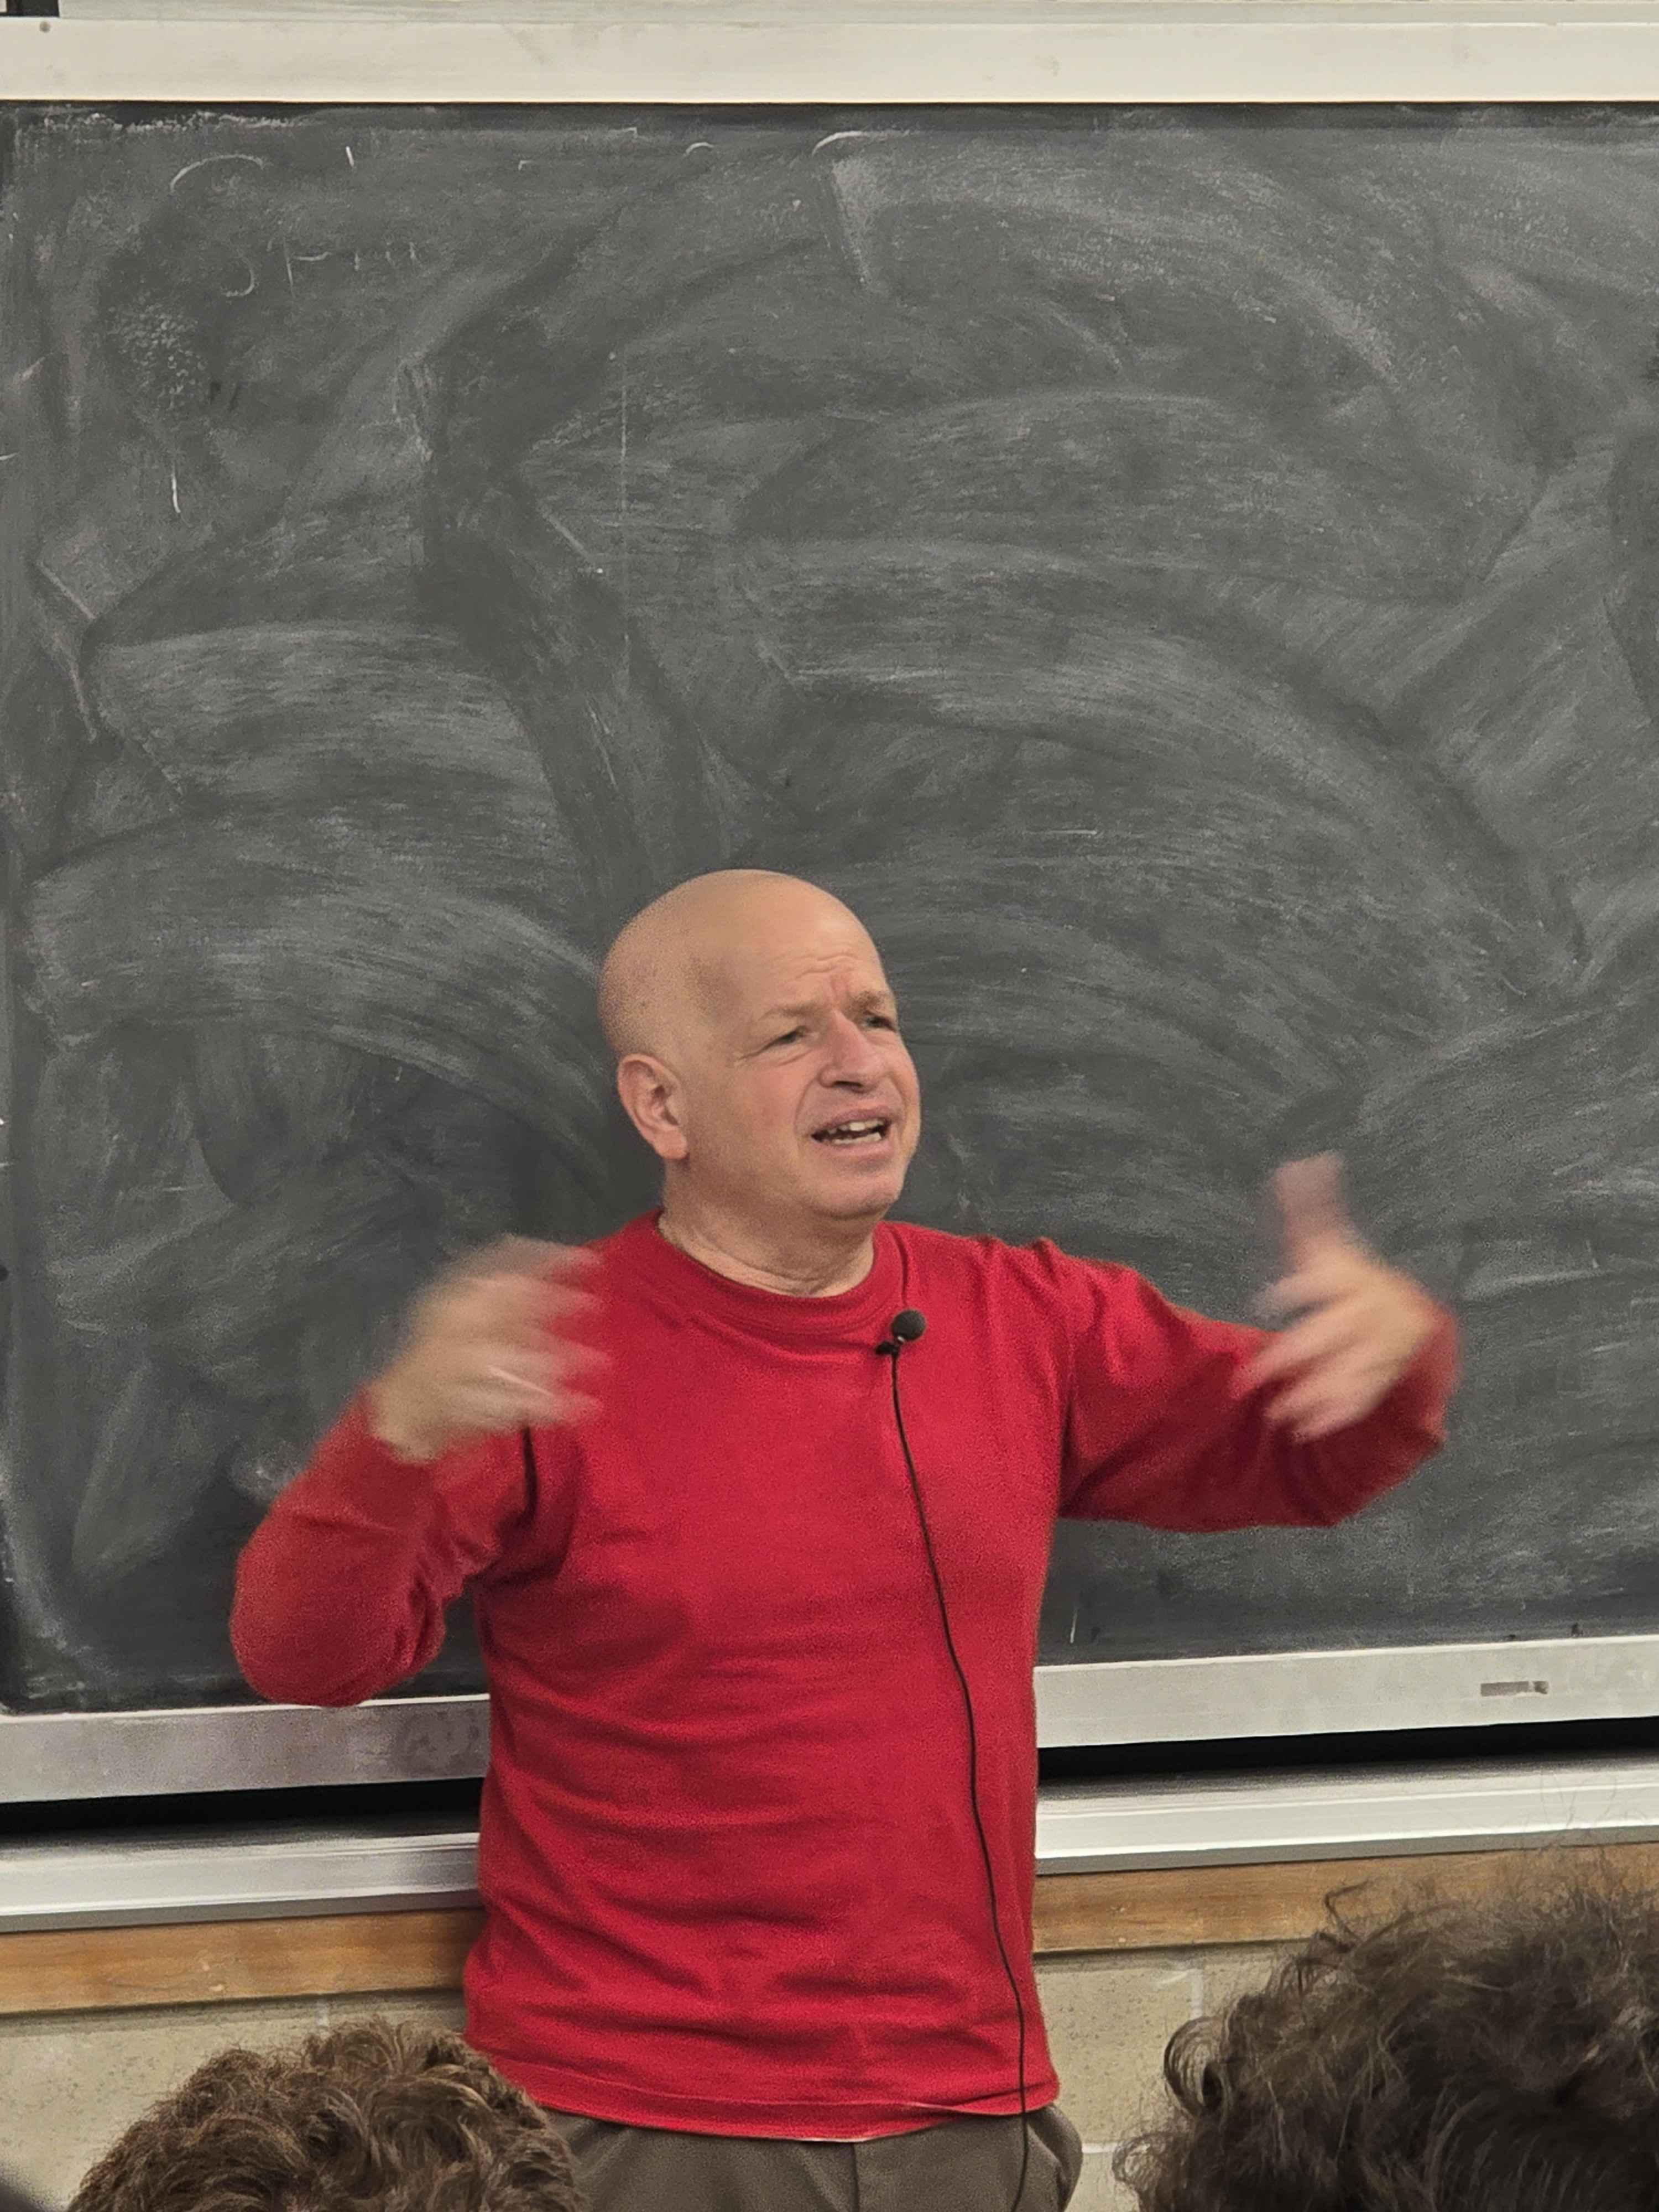
\includegraphics[scale=0.1]{MAT327 Notes/Dror Shirts/dror day 23 shirt.jpg}
\end{figure}

\noindent We start by defining functors. A functor $F : \SC \to \SD$ is a mapping between categories $\SC \to \SD$; it associates each $A \in \mathrm{obj}_{\SC}$ with an object $F(A) \in \mathrm{obj}_{\SD}$; in particular, we may draw the following diagram,
\[
    \begin{tikzcd}
        A \arrow[r, rightsquigarrow] \arrow[d, "f"'] \arrow[dd, bend right=40, "g \, \circ f"'] & FA \arrow[d, "Ff"] \arrow[dd, bend left=60, "Fg \, \circ Ff"] \\
        B \arrow[r, rightsquigarrow] \arrow[d, "g"'] & FB \arrow[d, "Fg"] \\
        C \arrow[r, rightsquigarrow] & FC
    \end{tikzcd}
\]
where $F : \mathrm{mor}_{\SC}(A, B) \to \mathrm{mor}_{\SD}(FA, FB)$ for any $A, B \in \mathrm{obj}_{\SC}$ such that whenever $f \in \mathrm{mor}_{\SC}(A, B)$ and $g \in \mathrm{mor}_{\SC}(B, C)$, we have that $F(g \circ f) = (F g) \circ (F f)$, and for any $A \in \mathrm{obj}_{\SC}$, $F(\id_A) = \id_{FA}$. We start with some lousy examples.
\begin{enumerate}[label=(\alph*)]
    \item The forgetful functor, $\mathrm{Forget} : \mathrm{Top} \to \mathrm{Set}$, where $\mathrm{Top}$ is the category of topological spaces, and $\mathrm{Set}$ is the category of sets, is a functor that ``forgets'' the structures it is applied on. i.e., we have $(X, \ST) \rightsquigarrow X$, a continuous function $f : X \to Y$ is mapped to a function $f : X \to Y$ (continuity not needed). Some other examples include
    \begin{align*}
        F_2 &: \mathrm{Grp} \to \mathrm{Set}, \\
        F_3 &: \mathrm{Vect} \to \mathrm{Set}, \\
        F_4 &: \mathrm{Top}_0 \to \mathrm{Top},
    \end{align*}
    where $\mathrm{Top}_0$ is the category of base spaces, and $F_4$ forgets the base point.

    \item Let us consider a functor $\hat{\underline{3}} : \mathrm{Set} \to \mathrm{Set}$, $A \rightsquigarrow A \times \underline{3}$, where $\underline{3} = \{1, 2, 3\}$. This particular functor applied to functions gives
    \[ \hat{\underline{3}}(F) : \hat{\underline{A}} \to \hat{\underline{B}}, \]
    i.e. $A \times \underline{3} \to B \times \underline{3}$, where $(\hat{\underline{3}} f) (a, \nu) = (F(a), \nu)$.
    
    \item Sophisticated example! Let $\ast : \mathrm{Vect} \to \mathrm{Vect}$ be a functor, mapping objects as follows, $V \to \ast V_i := V^\ast$. Given a linear transformation $L : V \to W \rightsquigarrow \ast L := L^\ast : W^\ast \to V^\ast$. Consider the contravariant functor $\SC \rightsquigarrow \SC^{\mathrm{op}}$, where $\mathrm{obj} \SC^{\mathrm{op}} = \mathrm{obj} \SC$, and $\mathrm{mor}_{\SC^{\mathrm{op}}} (A, B) = \mathrm{mor}_{\SC}(B, A)$; intuitively, this is just ``reversing the arrows''.
    
    \item Our main example: let $\pi_1 : \mathrm{Top}_0 \to \mathrm{Grp}$, i.e. $\pi_1$ is a functor from based topological spaces into groups, where $\pi_1$ assigns $(X, x_0)$ to $\pi_1(X, x_0)$. If we have a continuous map $f : (X, x_0) \to (Y, y_0)$, then there is a morphism $\pi_1 f = f_\ast : \pi_1(X, x) \to \pi_1(Y, y_0)$. In particular, $f_\ast [\gamma] := [f \circ \gamma]$, where $\gamma : I \to X$ and $f \circ \gamma : I \to Y$. The diagram is as follows;
    \[
        \begin{tikzcd}
            (X, x_0) \arrow[r, "\pi_1"] \arrow[d, "f"'] & \pi_1(X, x_0) \arrow[d, "\pi_1 f = f_\ast"] \\
            (Y, y_0) \arrow[r, "\pi_1"] & \pi_1(Y, y_0)
        \end{tikzcd}
    \]
\end{enumerate}

\noindent We now move onto retracts.
\begin{definition}
    Let $A \subset X$; a morphism $r : X \to A$ is called a \textit{retract} of $X$ to $A$ if $\restr{r}{A} = \id_A$. Specifically, $r \circ \iota_A = \restr{r}{A}$.\footnote{what}
\end{definition}
\noindent For example, a bigass fat $A$ mapping to a regular $A$ is an example of a retract. 
\begin{figure}[h]
    \centering
    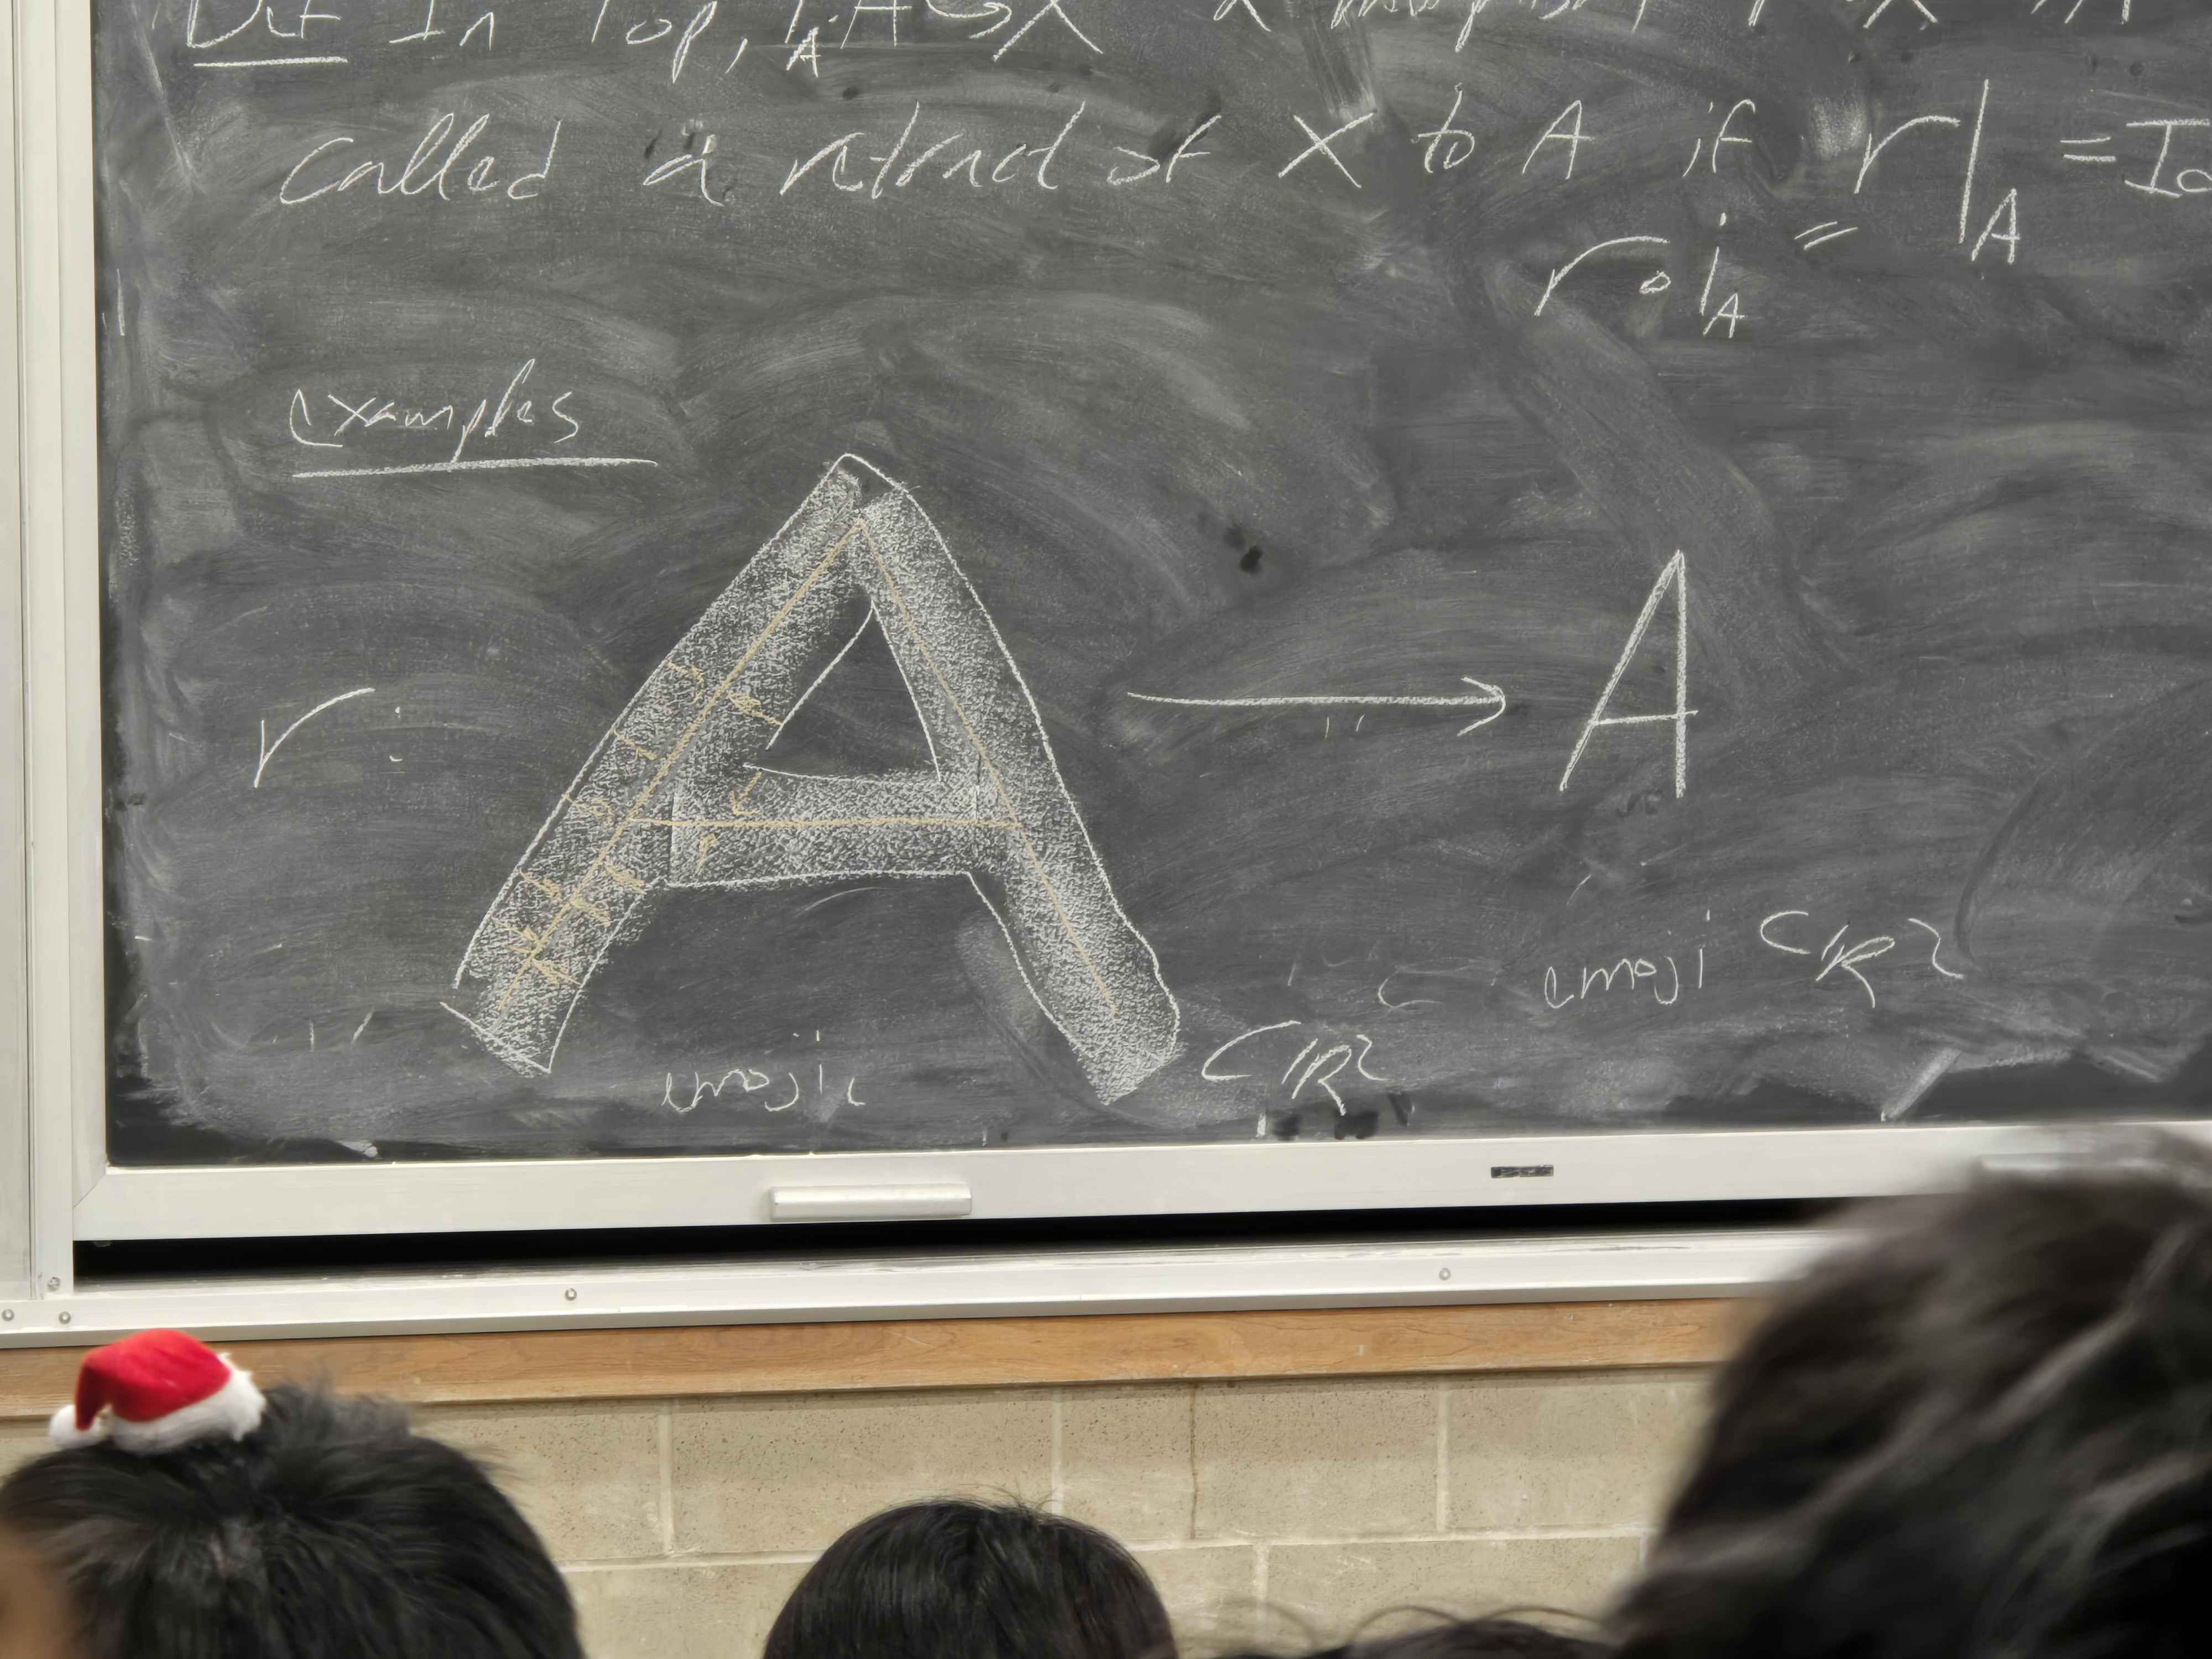
\includegraphics[scale=0.06]{MAT327 Notes/Blackboard Shots/Day 23 Retract.jpg}
\end{figure}

\newpage
\begin{simpleclaim}
    There does not exact a retract $r : D^1 \to S^0$.
\end{simpleclaim}
\noindent Recall that $D^n = \{x \in \RR^n \mid \abs{x} \leq 1\}$, and d$S^n = \{x \in \RR^{n+1} \mid \abs{x} = 1\}$. Informally, there is no way to do this without tearing $S^0$; formally, it is because of connectivity.
\medskip\newline
For next lecture, we will prove the following claim:
\begin{simpleclaim}
    There does not exist a retract $D^2 \to S^1$.
\end{simpleclaim}